\subsection{SOlUCIÓN 2}
	
	\begin{frame}{Solución de la actividad "Modificación de las variables de una señal periódica"}
	\begin{figure}[H]
		\vspace{-3mm}
		\centering 
		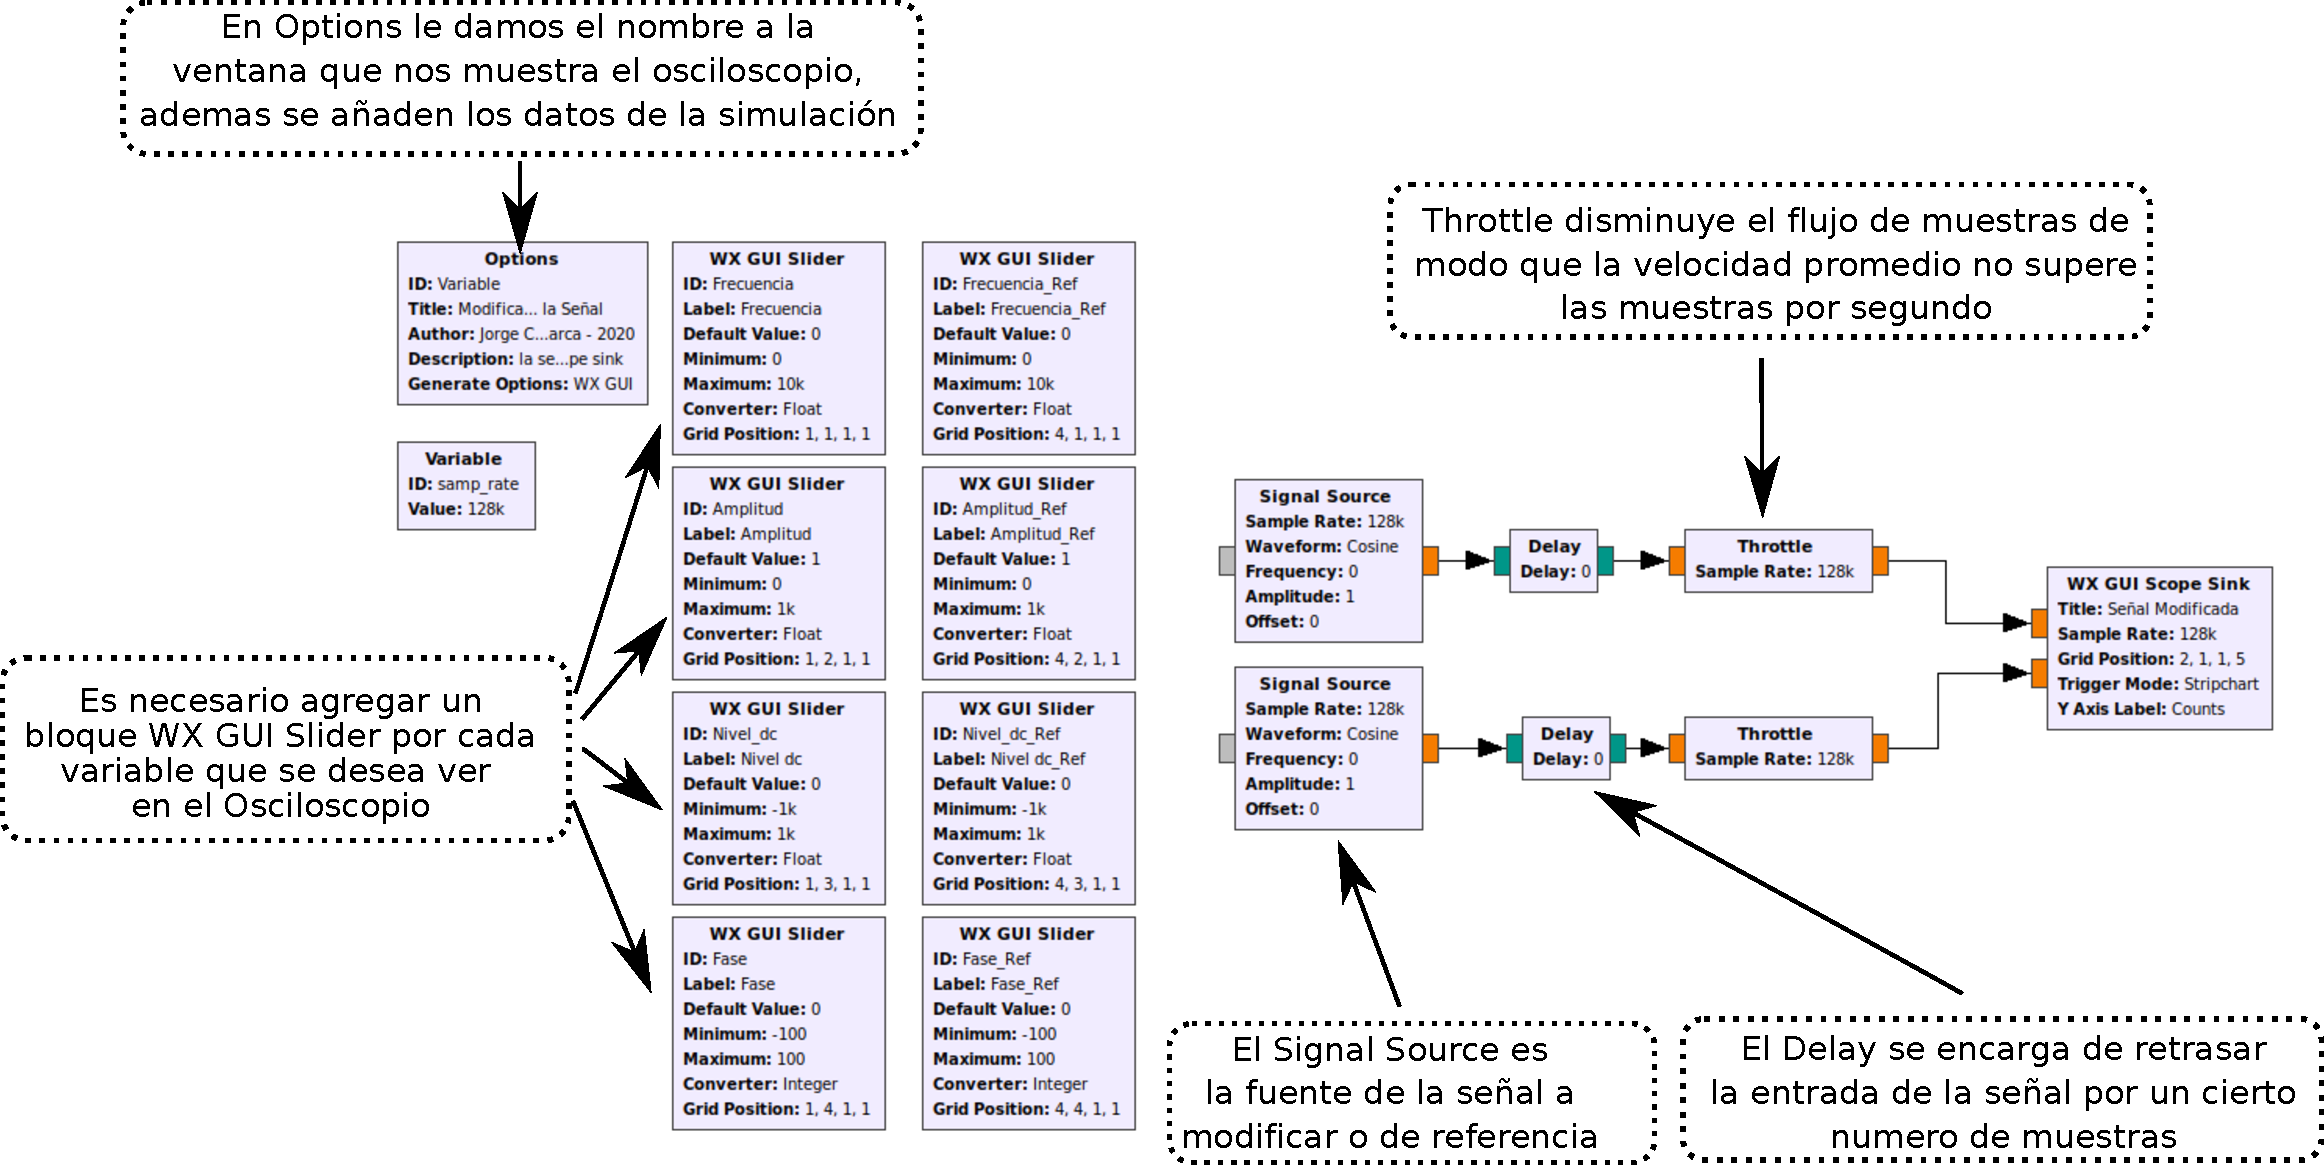
\includegraphics[width=0.9\textwidth]{soluciones/actividad_2/pdf/Mon.pdf}
		\end{figure}
	\end{frame}
	
	\begin{frame}
	\frametitle{\underline{\textbf{Solución de la actividad "Modificación de las variables de una señal periódica"}}}

	Los pasos son:
	\begin{enumerate}[1.]

	\item{En la presentación anterior, se pueden observar los WX GUI Slider para la frecuencia, la amplitud y el nivel DC. A su vez, se puede visualizar la configuración del bloque "Delay" para lograr el desfasamiento de la señal, como se muestra a continuación:}\\
	
	\end{enumerate}
	\end{frame}
	
	\begin{frame}{Solución de la actividad "Modificación de las variables de una señal periódica"}
	\begin{figure}[H]
		\vspace{-3mm}
		\centering
		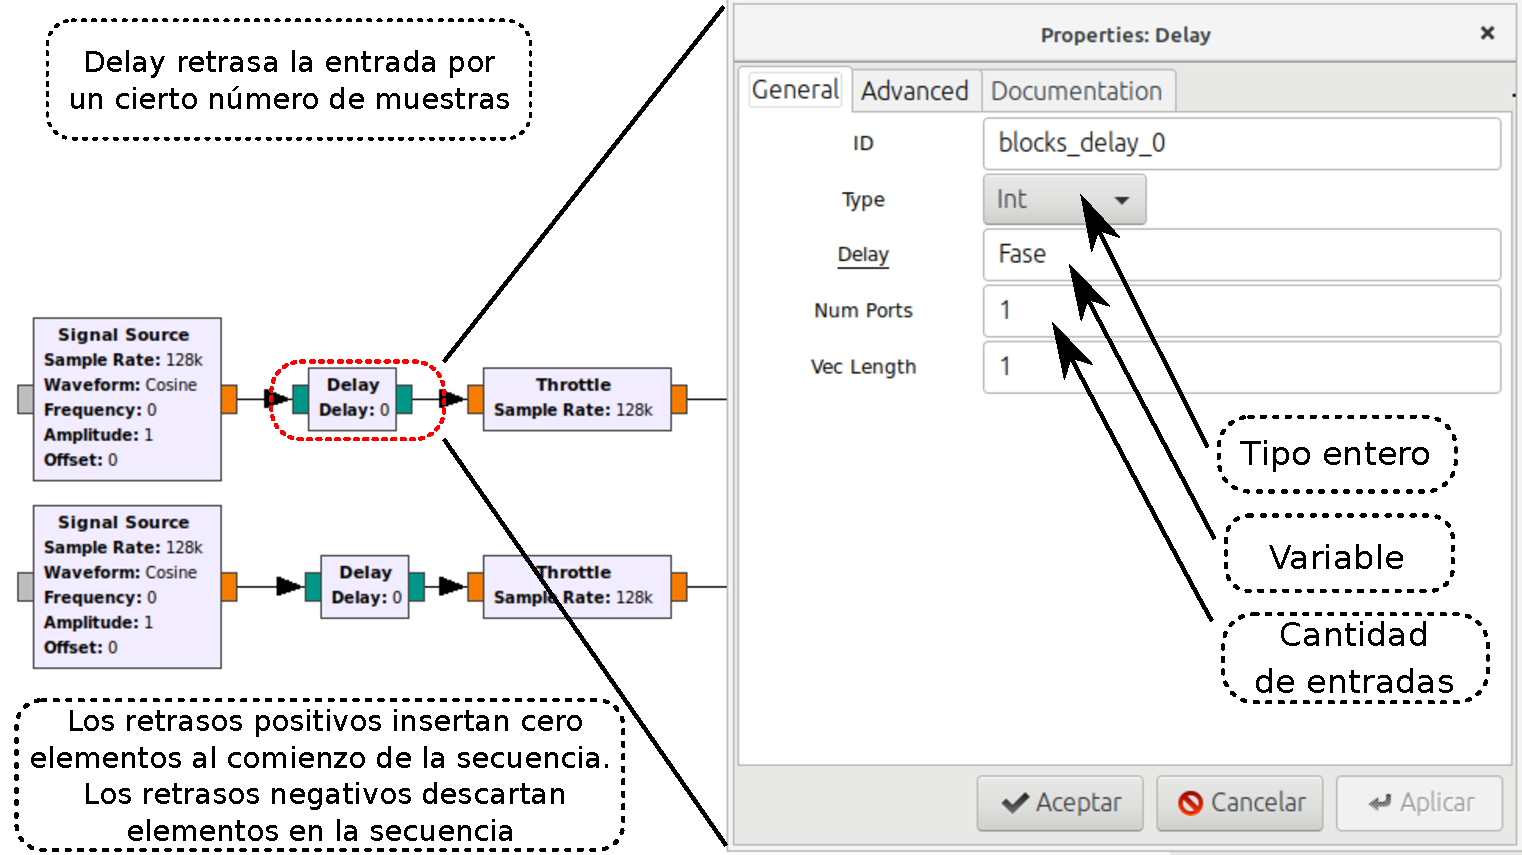
\includegraphics[width=0.9\textwidth]{soluciones/actividad_2/pdf/Delay.pdf}
		\end{figure}
	\end{frame}

	\begin{frame}
	\frametitle{\underline{\textbf{SSolución de la actividad "Modificación de las variables de una señal periódica"}}}
	\begin{enumerate}[2.]
	
	\item{Luego añadimos un WX GUI Slider para determinar la variación manual de la fase, donde se establece el ID de fase y los valores mínimos y máximos que puede tomar el retraso en fase.}\\
	\item{Lo que obtendremos al compilar el programa será el osciloscopio con las opciones adicionales de fijar los valores de amplitud, frecuencia, fase y nivel DC de la señal, tal y como se muestra a continuación:}\\
	
	\end{enumerate}
	\end{frame}


	\begin{frame}{Solución de la actividad}
	\begin{figure}[H]
		\vspace{-3mm}
		\centering
		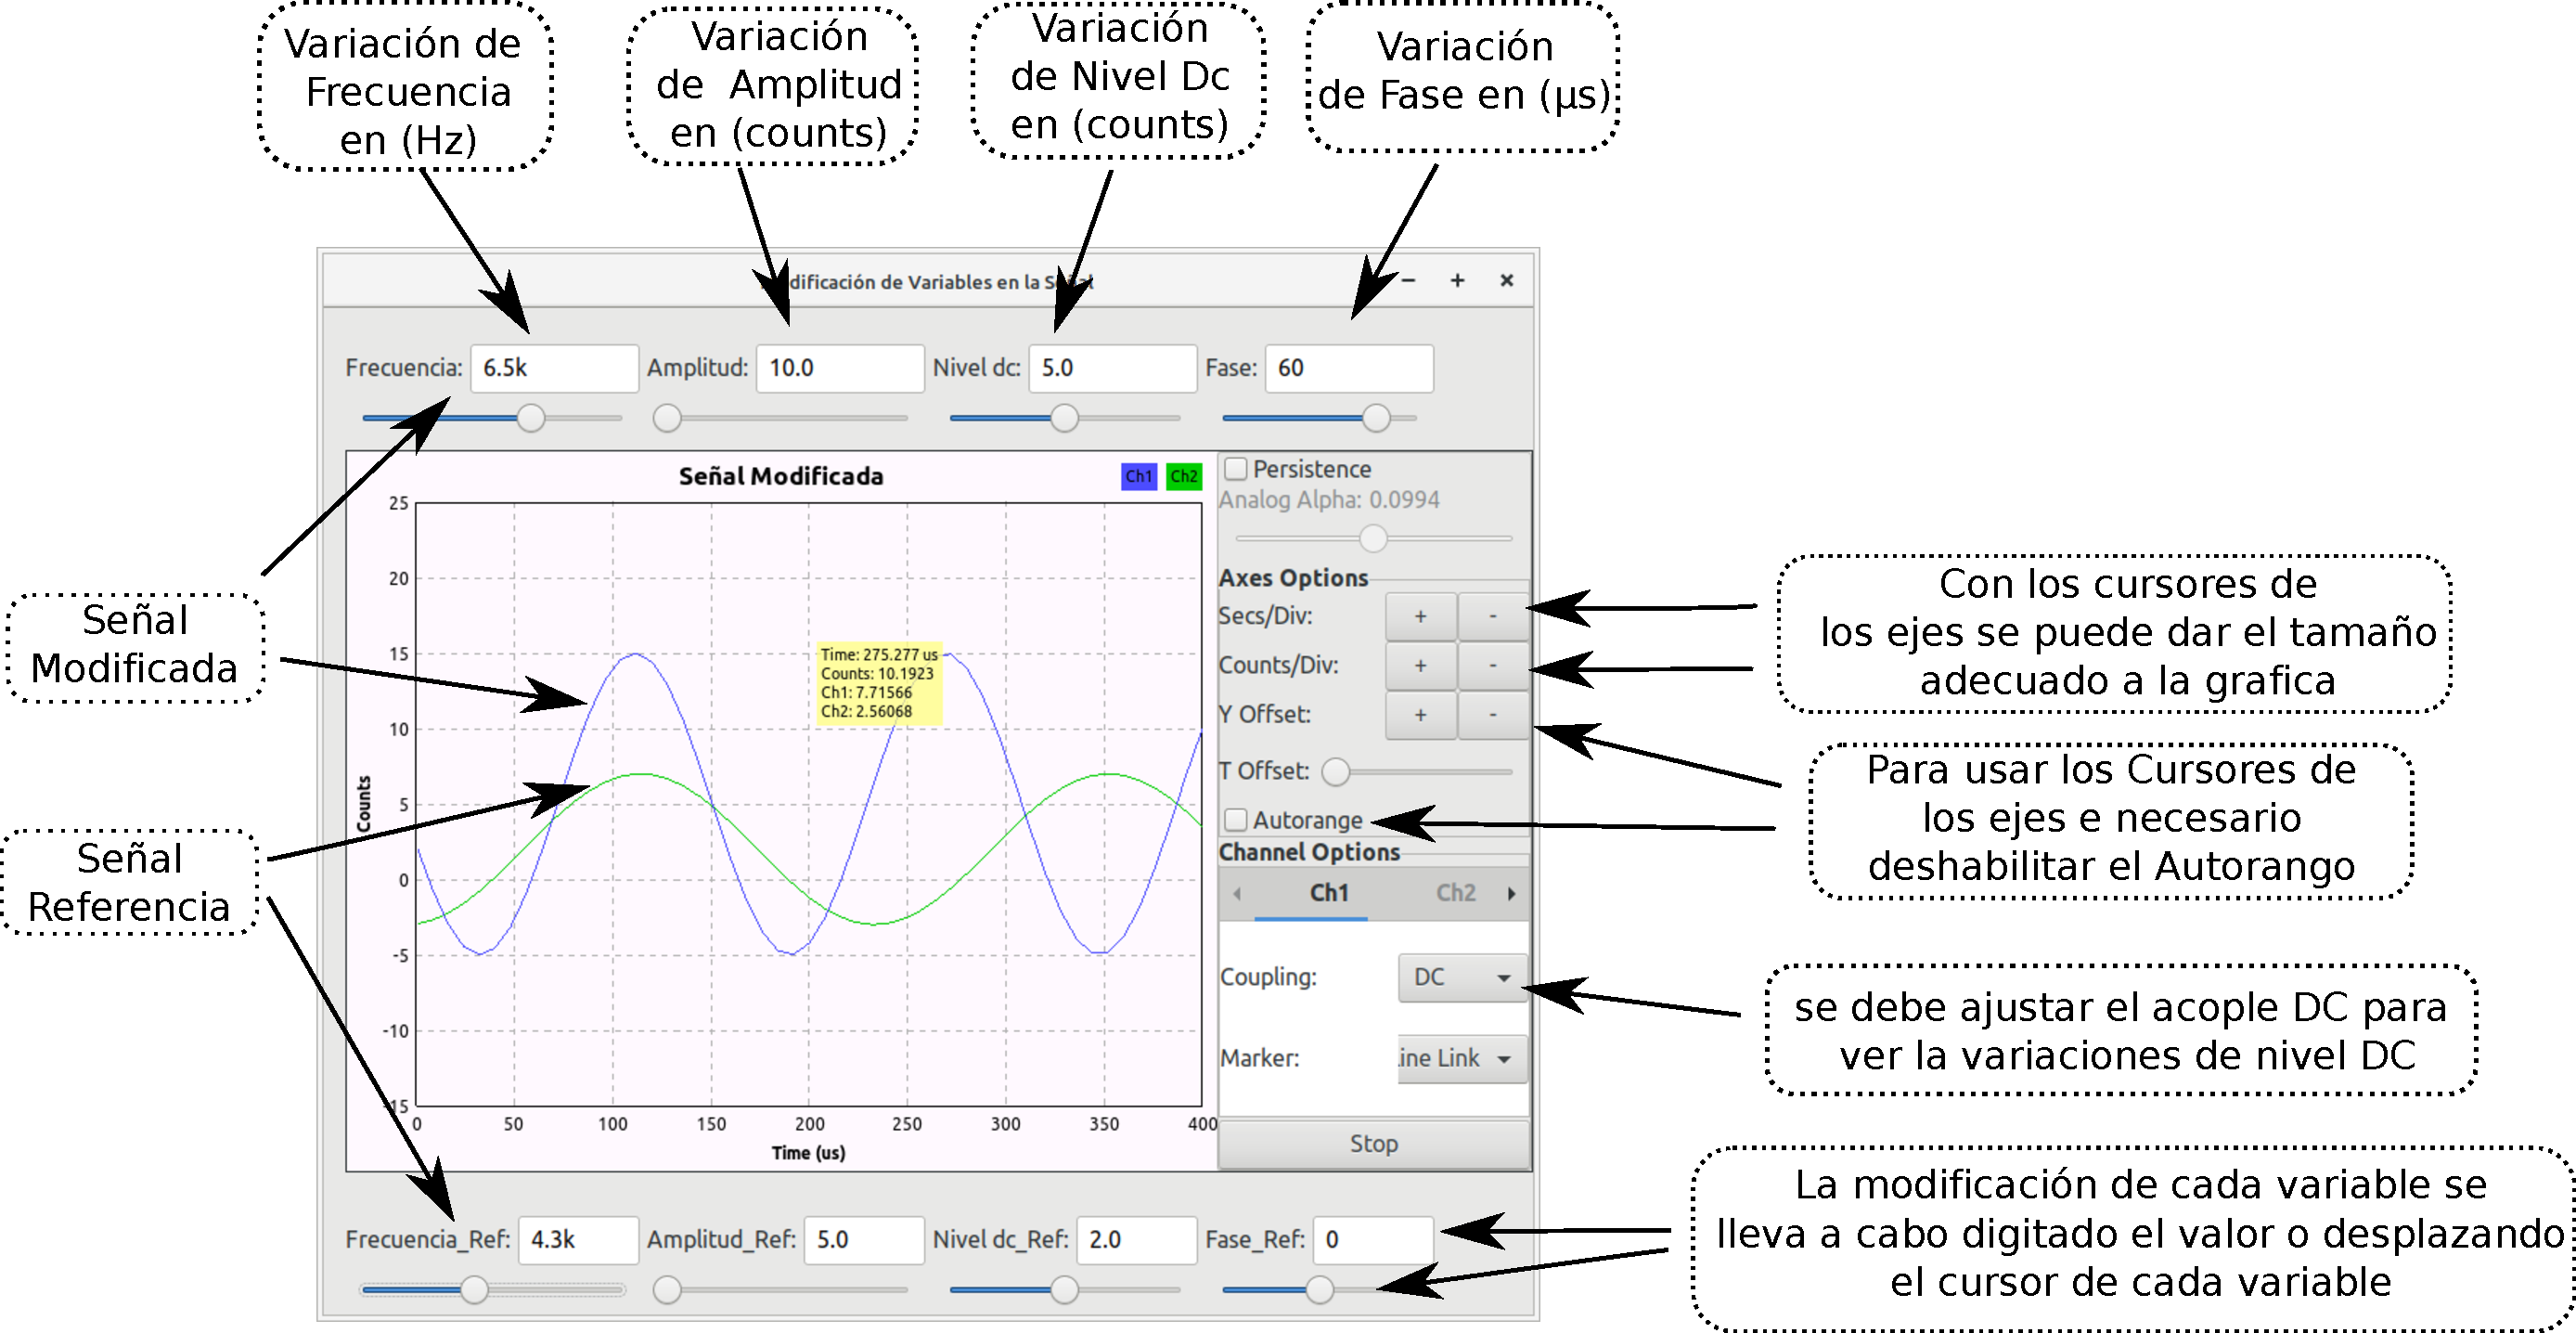
\includegraphics[width=0.9\textwidth]{soluciones/actividad_2/pdf/Salida.pdf}
		\end{figure}
	\end{frame}
	
	
